\documentclass{article}\usepackage[]{graphicx}\usepackage[]{color}
%% maxwidth is the original width if it is less than linewidth
%% otherwise use linewidth (to make sure the graphics do not exceed the margin)
\makeatletter
\def\maxwidth{ %
  \ifdim\Gin@nat@width>\linewidth
    \linewidth
  \else
    \Gin@nat@width
  \fi
}
\makeatother

\definecolor{fgcolor}{rgb}{0.345, 0.345, 0.345}
\newcommand{\hlnum}[1]{\textcolor[rgb]{0.686,0.059,0.569}{#1}}%
\newcommand{\hlstr}[1]{\textcolor[rgb]{0.192,0.494,0.8}{#1}}%
\newcommand{\hlcom}[1]{\textcolor[rgb]{0.678,0.584,0.686}{\textit{#1}}}%
\newcommand{\hlopt}[1]{\textcolor[rgb]{0,0,0}{#1}}%
\newcommand{\hlstd}[1]{\textcolor[rgb]{0.345,0.345,0.345}{#1}}%
\newcommand{\hlkwa}[1]{\textcolor[rgb]{0.161,0.373,0.58}{\textbf{#1}}}%
\newcommand{\hlkwb}[1]{\textcolor[rgb]{0.69,0.353,0.396}{#1}}%
\newcommand{\hlkwc}[1]{\textcolor[rgb]{0.333,0.667,0.333}{#1}}%
\newcommand{\hlkwd}[1]{\textcolor[rgb]{0.737,0.353,0.396}{\textbf{#1}}}%

\usepackage{framed}
\makeatletter
\newenvironment{kframe}{%
 \def\at@end@of@kframe{}%
 \ifinner\ifhmode%
  \def\at@end@of@kframe{\end{minipage}}%
  \begin{minipage}{\columnwidth}%
 \fi\fi%
 \def\FrameCommand##1{\hskip\@totalleftmargin \hskip-\fboxsep
 \colorbox{shadecolor}{##1}\hskip-\fboxsep
     % There is no \\@totalrightmargin, so:
     \hskip-\linewidth \hskip-\@totalleftmargin \hskip\columnwidth}%
 \MakeFramed {\advance\hsize-\width
   \@totalleftmargin\z@ \linewidth\hsize
   \@setminipage}}%
 {\par\unskip\endMakeFramed%
 \at@end@of@kframe}
\makeatother

\definecolor{shadecolor}{rgb}{.97, .97, .97}
\definecolor{messagecolor}{rgb}{0, 0, 0}
\definecolor{warningcolor}{rgb}{1, 0, 1}
\definecolor{errorcolor}{rgb}{1, 0, 0}
\newenvironment{knitrout}{}{} % an empty environment to be redefined in TeX

\usepackage{alltt}
\usepackage{alltt}
\usepackage{amsmath}
\usepackage[sc]{mathpazo}
\usepackage[T1]{fontenc}
\usepackage{geometry}
\geometry{verbose,tmargin=2.5cm,bmargin=2.5cm,lmargin=2.5cm,rmargin=2.5cm}
\setcounter{secnumdepth}{2}
\setcounter{tocdepth}{2}
\usepackage{url}
\usepackage[unicode=true,pdfusetitle,
 bookmarks=true,bookmarksnumbered=true,bookmarksopen=true,bookmarksopenlevel=2,
 breaklinks=false,pdfborder={0 0 1},backref=false,colorlinks=false]
 {hyperref}
\hypersetup{
 pdfstartview={XYZ null null 1}}
 
\title{Code for Supplementary Figure 2}
 
\usepackage{breakurl}
\IfFileExists{upquote.sty}{\usepackage{upquote}}{}
\begin{document}
\maketitle
%\SweaveOpts{concordance=TRUE}



\section{Create datasets}

Load the necessary libraries, source the file with the R functions:
\begin{knitrout}
\definecolor{shadecolor}{rgb}{0.969, 0.969, 0.969}\color{fgcolor}\begin{kframe}
\begin{alltt}
\hlkwd{library}\hlstd{(ggplot2)}

\hlkwd{source}\hlstd{(}\hlstr{"functions.R"}\hlstd{)}
\end{alltt}
\end{kframe}
\end{knitrout}

These results are for the $I=2, p=2$ case, so the parameters we vary are:
$r_1, r_2, \rho_{12,1}, \rho_{12,2}$. We save the relative efficiencies for both coefficients.
For Panel a), we take $\rho_{12,1} = 0, r_1=r_2=r$:
\begin{knitrout}
\definecolor{shadecolor}{rgb}{0.969, 0.969, 0.969}\color{fgcolor}\begin{kframe}
\begin{alltt}
\hlstd{bigMat.a} \hlkwb{<-} \hlkwd{expand.grid}\hlstd{(}\hlkwc{r}\hlstd{=}\hlkwd{c}\hlstd{(}\hlnum{0.1}\hlstd{,} \hlnum{0.5}\hlstd{,} \hlnum{0.9}\hlstd{),}
                        \hlkwc{rho121}\hlstd{=}\hlnum{0}\hlstd{,} \hlkwc{rho122}\hlstd{=(}\hlopt{-}\hlnum{19}\hlopt{:}\hlnum{19}\hlstd{)}\hlopt{/}\hlnum{20}\hlstd{)}
\hlstd{bigMat.a} \hlkwb{<-} \hlkwd{cbind}\hlstd{(bigMat.a,} \hlkwc{RelEff1}\hlstd{=}\hlnum{NA}\hlstd{,} \hlkwc{RelEff2}\hlstd{=}\hlnum{NA}\hlstd{)}
\hlstd{bigMat.a} \hlkwb{<-} \hlkwd{as.matrix}\hlstd{(bigMat.a)}
\hlkwa{for}\hlstd{(i} \hlkwa{in} \hlnum{1}\hlopt{:}\hlkwd{nrow}\hlstd{(bigMat.a))}
\hlstd{\{}
  \hlstd{rho121} \hlkwb{<-} \hlstd{bigMat.a[i,}\hlstr{"rho121"}\hlstd{]}
  \hlstd{rho122} \hlkwb{<-} \hlstd{bigMat.a[i,}\hlstr{"rho122"}\hlstd{]}
  \hlstd{r} \hlkwb{<-} \hlstd{bigMat.a[i,} \hlstr{"r"}\hlstd{]}

  \hlstd{bigMat.a[i,}\hlkwd{c}\hlstd{(}\hlnum{4}\hlstd{,}\hlnum{5}\hlstd{)]} \hlkwb{<-} \hlkwd{effCalc2}\hlstd{(}\hlkwc{rho112}\hlstd{=rho121,} \hlkwc{rho212}\hlstd{=rho122,} \hlkwc{r1}\hlstd{=r,} \hlkwc{r2}\hlstd{=r)}
\hlstd{\}}
\hlcom{##turn it back into data frame (need it as data frame for ggplot)}
\hlstd{bigMat.a} \hlkwb{<-} \hlkwd{as.data.frame}\hlstd{(bigMat.a)}
\hlcom{##check that relative efficiencies are identical for the two coefficients}
\hlkwd{identical}\hlstd{(bigMat.a}\hlopt{$}\hlstd{RelEff1, bigMat.a}\hlopt{$}\hlstd{RelEff2)}
\end{alltt}
\begin{verbatim}
## [1] TRUE
\end{verbatim}
\begin{alltt}
\hlcom{##rename RelEff1 as RelEff}
\hlkwd{names}\hlstd{(bigMat.a)[}\hlkwd{names}\hlstd{(bigMat.a)} \hlopt{==} \hlstr{"RelEff1"}\hlstd{]} \hlkwb{<-} \hlstr{"RelEff"}
\hlcom{##make r into a factor (needed for ggplot)}
\hlstd{bigMat.a}\hlopt{$}\hlstd{r} \hlkwb{<-} \hlkwd{paste}\hlstd{(}\hlstr{"r="}\hlstd{, bigMat.a}\hlopt{$}\hlstd{r,} \hlkwc{sep}\hlstd{=}\hlstr{""}\hlstd{)}\hlcom{##as.factor(bigMat.a$r)}
\end{alltt}
\end{kframe}
\end{knitrout}

For Panel b), we take $r_1 = 0.5, \rho_{12,1}=0.5$:
\begin{knitrout}
\definecolor{shadecolor}{rgb}{0.969, 0.969, 0.969}\color{fgcolor}\begin{kframe}
\begin{alltt}
\hlstd{bigMat.b} \hlkwb{<-} \hlkwd{expand.grid}\hlstd{(}\hlkwc{r1}\hlstd{=}\hlnum{1}\hlopt{/}\hlnum{2}\hlstd{,} \hlkwc{r2}\hlstd{=}\hlkwd{c}\hlstd{(}\hlnum{0.1}\hlstd{,} \hlnum{0.5}\hlstd{,} \hlnum{0.9}\hlstd{),}
                        \hlkwc{rho121}\hlstd{=}\hlnum{0.5}\hlstd{,} \hlkwc{rho122}\hlstd{=(}\hlopt{-}\hlnum{19}\hlopt{:}\hlnum{19}\hlstd{)}\hlopt{/}\hlnum{20}\hlstd{)}
\hlstd{bigMat.b} \hlkwb{<-} \hlkwd{cbind}\hlstd{(bigMat.b,} \hlkwc{RelEff1}\hlstd{=}\hlnum{0}\hlstd{,} \hlkwc{RelEff2}\hlstd{=}\hlnum{0}\hlstd{)}
\hlstd{bigMat.b} \hlkwb{<-} \hlkwd{as.matrix}\hlstd{(bigMat.b)}
\hlkwa{for}\hlstd{(i} \hlkwa{in} \hlnum{1}\hlopt{:}\hlkwd{nrow}\hlstd{(bigMat.b))}
\hlstd{\{}
  \hlstd{rho121} \hlkwb{<-} \hlstd{bigMat.b[i,}\hlstr{"rho121"}\hlstd{]}
  \hlstd{rho122} \hlkwb{<-} \hlstd{bigMat.b[i,}\hlstr{"rho122"}\hlstd{]}
  \hlstd{r1} \hlkwb{<-} \hlstd{bigMat.b[i,} \hlstr{"r1"}\hlstd{]}
  \hlstd{r2} \hlkwb{<-} \hlstd{bigMat.b[i,} \hlstr{"r2"}\hlstd{]}

  \hlstd{bigMat.b[i,}\hlkwd{c}\hlstd{(}\hlnum{5}\hlstd{,}\hlnum{6}\hlstd{)]} \hlkwb{<-} \hlkwd{effCalc2}\hlstd{(}\hlkwc{rho112}\hlstd{=rho121,} \hlkwc{rho212}\hlstd{=rho122,} \hlkwc{r1}\hlstd{=r1,} \hlkwc{r2}\hlstd{=r2)}
\hlstd{\}}
\hlcom{##turn it back into data frame (need it as data frame for ggplot)}
\hlstd{bigMat.b} \hlkwb{<-} \hlkwd{as.data.frame}\hlstd{(bigMat.b)}
\hlkwd{identical}\hlstd{(bigMat.b}\hlopt{$}\hlstd{RelEff1, bigMat.b}\hlopt{$}\hlstd{RelEff2)}
\end{alltt}
\begin{verbatim}
## [1] FALSE
\end{verbatim}
\begin{alltt}
\hlcom{##rename RelEff1 as RelEff}
\hlkwd{names}\hlstd{(bigMat.b)[}\hlkwd{names}\hlstd{(bigMat.b)} \hlopt{==} \hlstr{"RelEff1"}\hlstd{]} \hlkwb{<-} \hlstr{"RelEff"}
\hlcom{##make r2 into a factor (needed for ggplot)}
\hlstd{bigMat.b}\hlopt{$}\hlstd{r2} \hlkwb{<-} \hlkwd{as.factor}\hlstd{(bigMat.b}\hlopt{$}\hlstd{r2)}
\end{alltt}
\end{kframe}
\end{knitrout}

\section{Create plots}

Panel a):
\begin{knitrout}
\definecolor{shadecolor}{rgb}{0.969, 0.969, 0.969}\color{fgcolor}\begin{kframe}
\begin{alltt}
\hlstd{panelA} \hlkwb{<-} \hlkwd{ggplot}\hlstd{(bigMat.a,}
                 \hlkwd{aes}\hlstd{(}\hlkwc{x}\hlstd{=rho122,} \hlkwc{y}\hlstd{=RelEff))} \hlopt{+}
  \hlkwd{geom_line}\hlstd{(}\hlkwc{size}\hlstd{=}\hlnum{1.3}\hlstd{,} \hlkwd{aes}\hlstd{(}\hlkwc{linetype}\hlstd{=r,} \hlkwc{color}\hlstd{=r))} \hlopt{+}
  \hlkwd{theme_bw}\hlstd{(}\hlkwc{base_size} \hlstd{=} \hlnum{20}\hlstd{)}\hlopt{+}
  \hlkwd{xlab}\hlstd{(}\hlkwd{expression}\hlstd{(}\hlkwd{paste}\hlstd{(rho[}\hlnum{2}\hlstd{])))} \hlopt{+}
  \hlkwd{scale_color_discrete}\hlstd{(}\hlkwc{name} \hlstd{=} \hlstr{""}\hlstd{,}
                       \hlkwc{labels} \hlstd{=}
                         \hlkwd{c}\hlstd{(}\hlkwd{expression}\hlstd{(}\hlkwd{paste}\hlstd{(r[}\hlnum{2}\hlstd{],} \hlstr{"="}\hlstd{,}
                                            \hlnum{0.1}\hlstd{)),}
                           \hlkwd{expression}\hlstd{(}\hlkwd{paste}\hlstd{(r[}\hlnum{2}\hlstd{],} \hlstr{"="}\hlstd{,}
                                            \hlnum{0.5}\hlstd{)),}
                           \hlkwd{expression}\hlstd{(}\hlkwd{paste}\hlstd{(r[}\hlnum{2}\hlstd{],} \hlstr{"="}\hlstd{,}
                                            \hlnum{0.9}\hlstd{))))} \hlopt{+}
  \hlkwd{scale_linetype_discrete}\hlstd{(}\hlkwc{name} \hlstd{=} \hlstr{""}\hlstd{,}
                          \hlkwc{labels} \hlstd{=}
                            \hlkwd{c}\hlstd{(}\hlkwd{expression}\hlstd{(}\hlkwd{paste}\hlstd{(r[}\hlnum{2}\hlstd{],} \hlstr{"="}\hlstd{,}
                                               \hlnum{0.1}\hlstd{)),}
                              \hlkwd{expression}\hlstd{(}\hlkwd{paste}\hlstd{(r[}\hlnum{2}\hlstd{],} \hlstr{"="}\hlstd{,}
                                               \hlnum{0.5}\hlstd{)),}
                              \hlkwd{expression}\hlstd{(}\hlkwd{paste}\hlstd{(r[}\hlnum{2}\hlstd{],} \hlstr{"="}\hlstd{,}
                                               \hlnum{0.9}\hlstd{))))} \hlopt{+}
  \hlkwd{theme}\hlstd{(}\hlkwc{axis.line} \hlstd{=} \hlkwd{element_line}\hlstd{(}\hlkwc{colour} \hlstd{=} \hlstr{"black"}\hlstd{),}
        \hlkwc{plot.title} \hlstd{=} \hlkwd{element_text}\hlstd{(}\hlkwc{size} \hlstd{=} \hlnum{16}\hlstd{,} \hlkwc{hjust} \hlstd{=} \hlnum{0.5}\hlstd{),}
        \hlkwc{panel.grid.major} \hlstd{=} \hlkwd{element_blank}\hlstd{(),}
        \hlkwc{panel.grid.minor} \hlstd{=} \hlkwd{element_blank}\hlstd{(),}
        \hlkwc{panel.border} \hlstd{=} \hlkwd{element_blank}\hlstd{(),}
        \hlkwc{panel.background} \hlstd{=} \hlkwd{element_blank}\hlstd{(),}
        \hlkwc{legend.key} \hlstd{=} \hlkwd{element_blank}\hlstd{(),}
        \hlkwc{axis.line.x} \hlstd{=} \hlkwd{element_line}\hlstd{(}\hlkwc{color}\hlstd{=}\hlstr{"black"}\hlstd{,} \hlkwc{size} \hlstd{=} \hlnum{0.5}\hlstd{),} \hlcom{##this is to show axes - bug in this version of ggplot2}
        \hlkwc{axis.line.y} \hlstd{=} \hlkwd{element_line}\hlstd{(}\hlkwc{color}\hlstd{=}\hlstr{"black"}\hlstd{,} \hlkwc{size} \hlstd{=} \hlnum{0.5}\hlstd{))} \hlopt{+}
  \hlkwd{labs}\hlstd{(}\hlkwc{title}\hlstd{=}\hlkwd{expression}\hlstd{(}\hlkwd{atop}\hlstd{(}\hlstr{"(a)"}\hlstd{,} \hlkwd{paste}\hlstd{(}\hlstr{"Fixed effects: I = 2, "}\hlstd{,}
                                          \hlstd{rho[}\hlnum{1}\hlstd{],} \hlstr{" = "}\hlstd{,} \hlnum{0}\hlstd{,} \hlstr{", "}\hlstd{,}
                                          \hlstd{r[}\hlnum{1}\hlstd{],} \hlstr{" = "}\hlstd{, r[}\hlnum{2}\hlstd{]))))}
\end{alltt}
\end{kframe}
\end{knitrout}

Panel b):
\begin{knitrout}
\definecolor{shadecolor}{rgb}{0.969, 0.969, 0.969}\color{fgcolor}\begin{kframe}
\begin{alltt}
\hlstd{panelB} \hlkwb{<-} \hlkwd{ggplot}\hlstd{(bigMat.b,}
                 \hlkwd{aes}\hlstd{(}\hlkwc{x}\hlstd{=rho122,} \hlkwc{y}\hlstd{=RelEff))} \hlopt{+}
  \hlkwd{geom_line}\hlstd{(}\hlkwc{size}\hlstd{=}\hlnum{1.3}\hlstd{,} \hlkwd{aes}\hlstd{(}\hlkwc{linetype}\hlstd{=r2,} \hlkwc{color}\hlstd{=r2))} \hlopt{+}
  \hlkwd{theme_bw}\hlstd{(}\hlkwc{base_size} \hlstd{=} \hlnum{20}\hlstd{)} \hlopt{+}
  \hlkwd{xlab}\hlstd{(}\hlkwd{expression}\hlstd{(}\hlkwd{paste}\hlstd{(rho[}\hlnum{2}\hlstd{])))} \hlopt{+}
  \hlkwd{scale_color_discrete}\hlstd{(}\hlkwc{name} \hlstd{=} \hlstr{""}\hlstd{,}
                       \hlkwc{labels} \hlstd{=}
                         \hlkwd{c}\hlstd{(}\hlkwd{expression}\hlstd{(}\hlkwd{paste}\hlstd{(r[}\hlnum{2}\hlstd{],} \hlstr{"="}\hlstd{,}
                                            \hlnum{0.1}\hlstd{)),}
                           \hlkwd{expression}\hlstd{(}\hlkwd{paste}\hlstd{(r[}\hlnum{2}\hlstd{],} \hlstr{"="}\hlstd{,}
                                            \hlnum{0.5}\hlstd{)),}
                           \hlkwd{expression}\hlstd{(}\hlkwd{paste}\hlstd{(r[}\hlnum{2}\hlstd{],} \hlstr{"="}\hlstd{,}
                                            \hlnum{0.9}\hlstd{))))} \hlopt{+}
  \hlkwd{scale_linetype_discrete}\hlstd{(}\hlkwc{name} \hlstd{=} \hlstr{""}\hlstd{,}
                          \hlkwc{labels} \hlstd{=}
                            \hlkwd{c}\hlstd{(}\hlkwd{expression}\hlstd{(}\hlkwd{paste}\hlstd{(r[}\hlnum{2}\hlstd{],} \hlstr{"="}\hlstd{,}
                                               \hlnum{0.1}\hlstd{)),}
                              \hlkwd{expression}\hlstd{(}\hlkwd{paste}\hlstd{(r[}\hlnum{2}\hlstd{],} \hlstr{"="}\hlstd{,}
                                               \hlnum{0.5}\hlstd{)),}
                              \hlkwd{expression}\hlstd{(}\hlkwd{paste}\hlstd{(r[}\hlnum{2}\hlstd{],} \hlstr{"="}\hlstd{,}
                                               \hlnum{0.9}\hlstd{))))} \hlopt{+}
  \hlkwd{theme}\hlstd{(}\hlkwc{axis.line} \hlstd{=} \hlkwd{element_line}\hlstd{(}\hlkwc{colour} \hlstd{=} \hlstr{"black"}\hlstd{),}
        \hlkwc{plot.title} \hlstd{=} \hlkwd{element_text}\hlstd{(}\hlkwc{size} \hlstd{=} \hlnum{16}\hlstd{,} \hlkwc{hjust} \hlstd{=} \hlnum{0.5}\hlstd{),}
        \hlkwc{panel.grid.major} \hlstd{=} \hlkwd{element_blank}\hlstd{(),}
        \hlkwc{panel.grid.minor} \hlstd{=} \hlkwd{element_blank}\hlstd{(),}
        \hlkwc{panel.border} \hlstd{=} \hlkwd{element_blank}\hlstd{(),}
        \hlkwc{panel.background} \hlstd{=} \hlkwd{element_blank}\hlstd{(),}
        \hlkwc{legend.key} \hlstd{=} \hlkwd{element_blank}\hlstd{(),}
        \hlkwc{axis.line.x} \hlstd{=} \hlkwd{element_line}\hlstd{(}\hlkwc{color}\hlstd{=}\hlstr{"black"}\hlstd{,} \hlkwc{size} \hlstd{=} \hlnum{0.5}\hlstd{),} \hlcom{##this is to show axes - bug in this version of ggplot2}
        \hlkwc{axis.line.y} \hlstd{=} \hlkwd{element_line}\hlstd{(}\hlkwc{color}\hlstd{=}\hlstr{"black"}\hlstd{,} \hlkwc{size} \hlstd{=} \hlnum{0.5}\hlstd{))} \hlopt{+}
  \hlkwd{labs}\hlstd{(}\hlkwc{title}\hlstd{=}\hlkwd{expression}\hlstd{(}\hlkwd{atop}\hlstd{(}\hlstr{"(b)"}\hlstd{,} \hlkwd{paste}\hlstd{(}\hlstr{"Fixed effects: I = 2, "}\hlstd{,}
                                          \hlstd{rho[}\hlnum{1}\hlstd{],} \hlstr{" = "}\hlstd{,} \hlnum{0.5}\hlstd{,} \hlstr{", "}\hlstd{,}
                                          \hlstd{r[}\hlnum{1}\hlstd{],} \hlstr{" = "}\hlstd{,} \hlnum{0.5}\hlstd{))))}
\end{alltt}
\end{kframe}
\end{knitrout}

\section{Put both panels together}

\begin{knitrout}
\definecolor{shadecolor}{rgb}{0.969, 0.969, 0.969}\color{fgcolor}\begin{kframe}
\begin{alltt}
\hlkwd{multiplot}\hlstd{(panelA, panelB,} \hlkwc{cols}\hlstd{=}\hlnum{2}\hlstd{)}
\end{alltt}


{\ttfamily\noindent\itshape\color{messagecolor}{\#\# Loading required package: grid}}\end{kframe}

{\centering 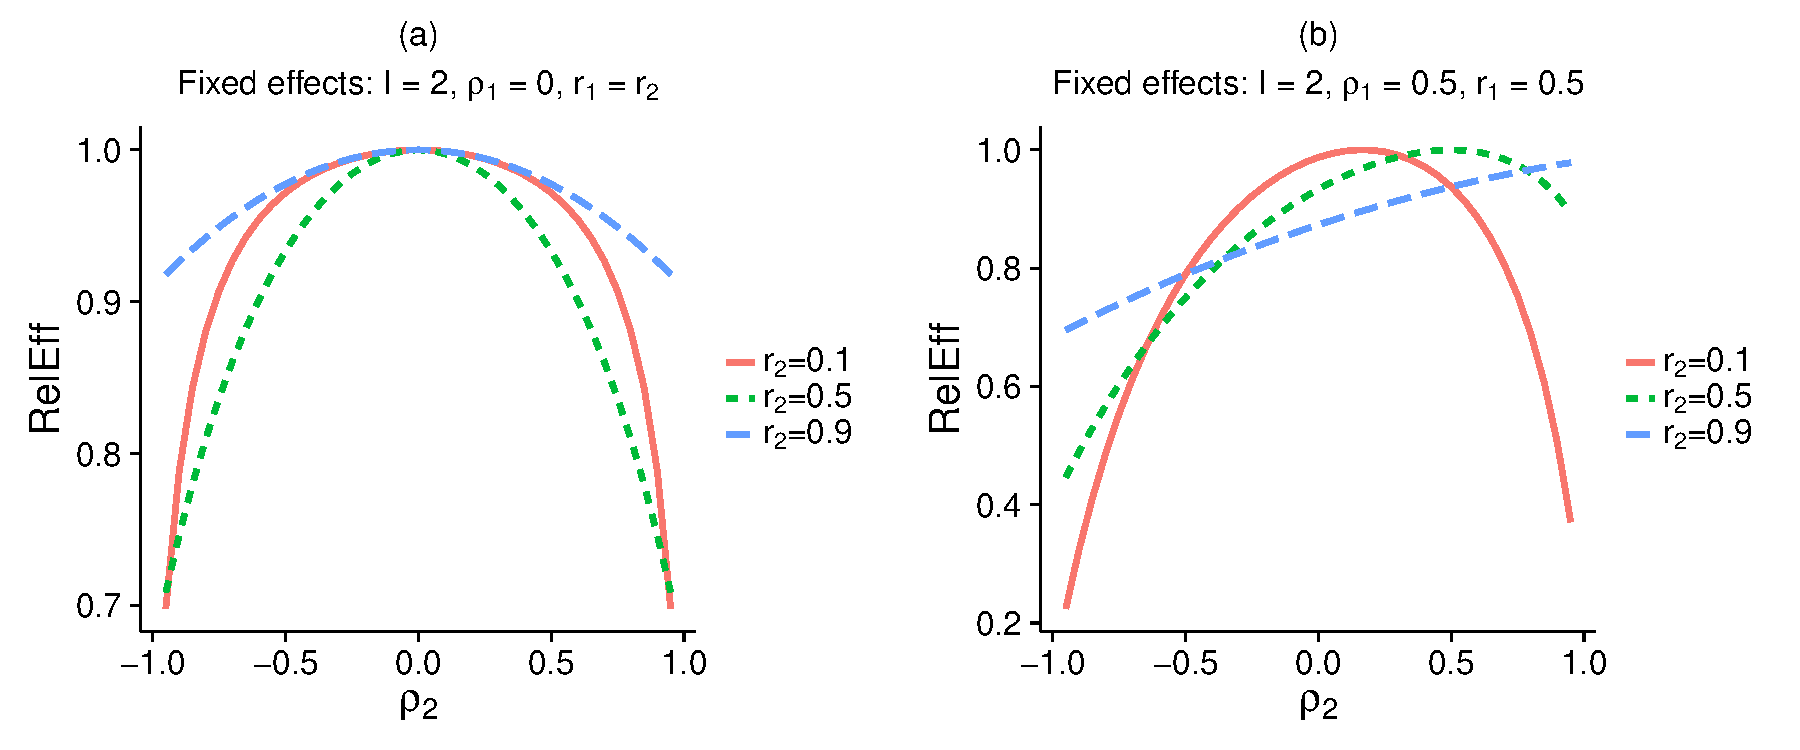
\includegraphics[width=\maxwidth]{figures/Figure_S2_panels_ab-1} 

}



\end{knitrout}



\end{document}











